\documentclass{article}
% Chinese
% \documentclass[UTF8, nofonts, mathptmx, 12pt, onecolumn]{article}
% \usepackage{xeCJK}
% \setCJKmainfont{SimSun}
\usepackage{amsmath}
\usepackage{amsfonts}
\usepackage{amssymb}
\usepackage{wasysym}
% \usepackage{ctex}
\usepackage{graphicx}
\usepackage{float}
\usepackage{geometry}
\geometry{a4paper,scale=0.8}
\usepackage{caption}
\usepackage{subcaption}
% \newcommand{\oiint}{\mathop{{\int\!\!\!\!\!\int}\mkern-21mu \bigcirc} {}}
\newcommand*{\dif}{\mathop{}\!\mathrm{d}}
\newcommand*{\md}{\mathop{}\!\mathrm{d}}
\newcommand*{\me}{\mathrm{e}}

\usepackage{parskip}
\setlength{\parindent}{0cm}

\usepackage{bm}
\let\Oldmathbf\mathbf
\renewcommand{\mathbf}[1]{\boldsymbol{\Oldmathbf{#1}}}
\let\eqnarray\align

\renewcommand*{\arraystretch}{2}
\usepackage{units}
\renewcommand{\frac}{\nicefrac}

\usepackage{cellspace}
\setlength{\cellspacetoplimit}{5pt}
\setlength{\cellspacebottomlimit}{5pt}

\author{Xiping Hu}
\usepackage{authblk}
\author{Xiping Hu}
\affil{https://hxp.plus/}
\title{Homework for Chapter 5}

\begin{document}
\maketitle

\begin{figure}[H]
  \centering
  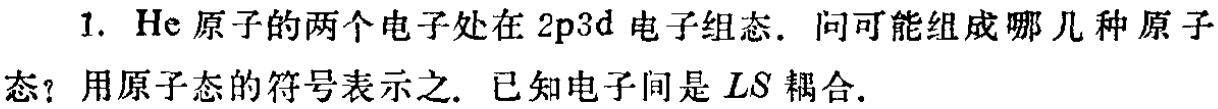
\includegraphics[width=\linewidth]{figures/Problem1}
  \label{fig:}
\end{figure}

\begin{equation*}
  \left\{
  \begin{aligned}
    & s_1 = s_2 = \dfrac{1}{2} \\
    & l_1 = 1 \\
    & l_2 = 2
  \end{aligned}
  \right.
  \Rightarrow
  \left\{
  \begin{aligned}
    & L = 3, 2, 1 \\
    & S = 1, 0
  \end{aligned}
  \right.
\end{equation*}

So that the atom has the following 12 states

\begin{center}
\begin{tabular}{ c|cc } 
        & S = 0 & S = 1 \\
  \hline
  L = 1 & ${}^{1}P_{1}$ & ${}^{3}P_{0,1,2}$ \\ 
  L = 2 & ${}^{1}D_{2}$ & ${}^{3}D_{1,2,3}$ \\
  L = 3 & ${}^{1}F_{3}$ & ${}^{3}F_{2,3,4}$ \\
\end{tabular}
\end{center}

\begin{figure}[H]
  \centering
  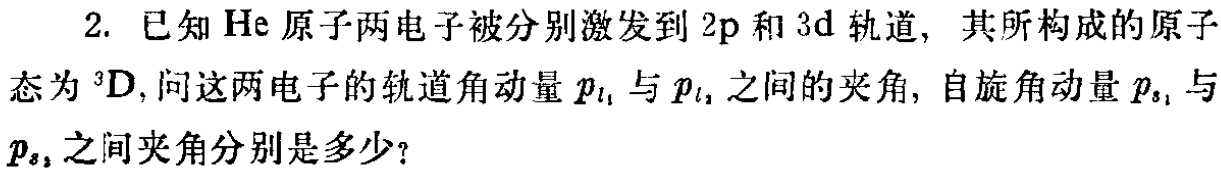
\includegraphics[width=\linewidth]{figures/Problem2}
  \label{fig:}
\end{figure}

\begin{equation*}
  \left\{
    \begin{aligned}
      & L = 2 \\
      & S = 1 \\
      & l_1 = 1 \\
      & l_2 = 2
    \end{aligned}
  \right.
  \Rightarrow
 \left\{
    \begin{aligned}
      & p_{l1} = \sqrt{l_1 \left( l_1 + 1 \right)} \hbar  = \sqrt{2} \hbar \\
      & p_{l2} = \sqrt{l_2 \left( l_2 + 1 \right)} \hbar = \sqrt{6} \hbar \\
      & P_l = \sqrt{L \left( L + 1 \right)} \hbar = \sqrt{6} \hbar
    \end{aligned}
  \right.
\end{equation*}

\begin{equation*}
  \begin{aligned}
    P_L^2 = p_{l1}^2 + p_{l2}^2 + 2 p_{l1} p_{l2} \cos \theta \Rightarrow \cos \theta = \dfrac{P_L^2 - p_{l1}^2 - p_{l2}^2}{2 p_{l1} p_{l2}} \Rightarrow \theta = 106^{\circ}
  \end{aligned}
\end{equation*}

\begin{figure}[H]
  \centering
  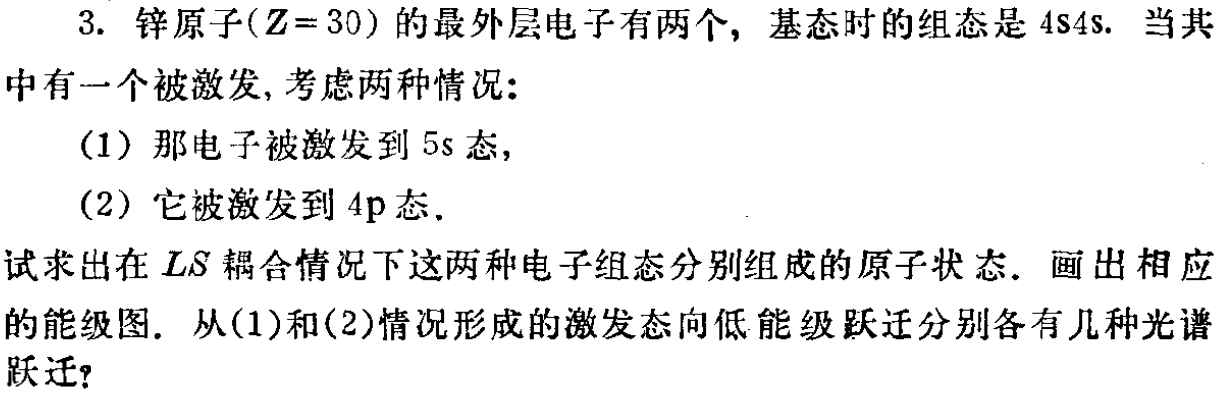
\includegraphics[width=\linewidth]{figures/Problem3}
  \label{fig:}
\end{figure}

\paragraph{Q1}

When the electrons is in 4s5s

\begin{equation*}
  \left\{
    \begin{aligned}
      & s_1 = s_2 = \dfrac{1}{2} \\
      & l_1 = 0 \\
      & l_2 = 0
    \end{aligned}
  \right.
  \Rightarrow
 \left\{
    \begin{aligned}
      & S = 0,1 \\
      & L = 0
    \end{aligned}
  \right.
\end{equation*}


\begin{center}
\begin{tabular}{ c|cc } 
        & S = 0 & S = 1 \\
  \hline
  L = 0 & ${}^{1}S_{0}$ & ${}^{3}S_{1}$ \\
  L = 1 & ${}^{1}P_{1}$ & ${}^{3}P_{0,1,2}$ 
\end{tabular}
\end{center}

The possible transitions are

\begin{equation*}
  \begin{aligned}
    & 5^1 S_0 \rightarrow 4^1 P_1 \\
    & 5^3 S_1 \rightarrow 4^3 P_0 \\
    & 5^3 S_1 \rightarrow 4^3 P_1 \\
    & 5^3 S_1 \rightarrow 4^3 P_2 \\
    & 4^3 P_2 \rightarrow 4^3 S_1 \\
  \end{aligned}
\end{equation*}

\paragraph{Q2}

When the electrons is in 4s5p

\begin{equation*}
  \left\{
    \begin{aligned}
      & s_1 = s_2 = \dfrac{1}{2} \\
      & l_1 = 0 \\
      & l_2 = 1
    \end{aligned}
  \right.
  \Rightarrow
 \left\{
    \begin{aligned}
      & S = 0,1 \\
      & L = 0,1
    \end{aligned}
  \right.
\end{equation*}

\begin{center}
\begin{tabular}{ c|cc } 
        & S = 0 & S = 1 \\
  \hline
  L = 0 & ${}^{1}S_{0}$ & ${}^{3}S_{1}$ \\
  L = 1 & ${}^{1}P_{1}$ & ${}^{3}P_{0,1,2}$ 
\end{tabular}
\end{center}

The possible transitions are

\begin{equation*}
  \begin{aligned}
    & 4^1 P_1 \rightarrow 4^1 S_0
  \end{aligned}
\end{equation*}

\begin{figure}[H]
  \centering
  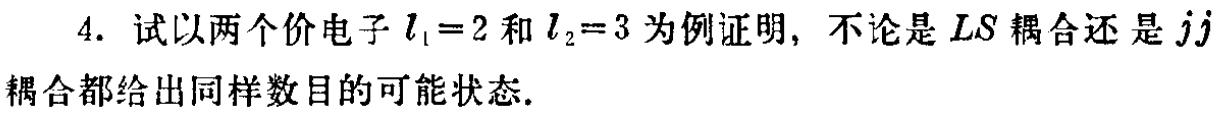
\includegraphics[width=\linewidth]{figures/Problem4}
  \label{fig:}
\end{figure}

L-S coupling has 20 states

\begin{equation*}
  \begin{aligned}
    & S = 0,1 \\
    & L = 1,2,3,4,5
  \end{aligned}
\end{equation*}

\begin{center}
\begin{tabular}{ c|cc } 
        & S = 0 & S = 1 \\
  \hline
  L = 1 & ${}^{1}P_{1}$ & ${}^{3}P_{0,1,2}$ \\ 
  L = 2 & ${}^{1}D_{2}$ & ${}^{3}D_{1,2,3}$ \\
  L = 3 & ${}^{1}F_{3}$ & ${}^{3}F_{2,3,4}$ \\
  L = 4 & ${}^{1}G_{4}$ & ${}^{3}G_{3,4,5}$ \\ 
  L = 5 & ${}^{1}H_{5}$ & ${}^{3}H_{4,5,6}$ \\ 
\end{tabular}
\end{center}

jj coupling has 20 states as follows, as well

\begin{center}
\begin{tabular}{ Sc|ScSc } 
        & $j_1 = \dfrac{5}{2} $ & $j_1 = \dfrac{3}{2} $ \\
  \hline
  $j_2 = \dfrac{7}{2} $ & $J = 6,5,4,3,2,1$ & $J = 5,4,3,2$ \\ 
  $j_2 = \dfrac{5}{2} $ & $J = 5,4,3,2,1,0$ & $J = 4,3,2,1$
\end{tabular}
\end{center}

\begin{figure}[H]
  \centering
  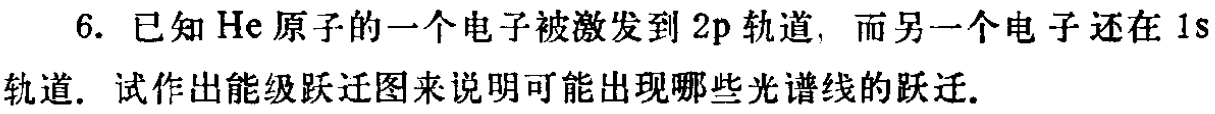
\includegraphics[width=\linewidth]{figures/Problem6}
  \label{fig:}
\end{figure}

\begin{equation*}
  \left\{
  \begin{aligned}
    & s_1 = s_2 = \dfrac{1}{2} \\
    & l_1 = 1 \\
    & l_2 = 0
  \end{aligned}
  \right.
  \Rightarrow
  \left\{
  \begin{aligned}
    & L = 1 \\
    & S = 1, 0
  \end{aligned}
  \right.
\end{equation*}

So that the atom has the following 12 states

\begin{center}
\begin{tabular}{ c|cc } 
        & S = 0 & S = 1 \\
  \hline
  L = 0 & ${}^{1}S_{0}$ & ${}^{3}S_{1}$ \\
  L = 1 & ${}^{1}P_{1}$ & ${}^{3}P_{0,1,2}$ \\ 
\end{tabular}
\end{center}

The possible transitions are

\begin{equation*}
  \begin{aligned}
    & 2^1 P_1 \rightarrow 1^1 S_0 \\
    & 2^1 P_1 \rightarrow 2^1 S_0 \\
    & 2^3 P_0 \rightarrow 2^3 S_1 \\
    & 2^3 P_1 \rightarrow 2^3 S_1 \\
    & 2^3 P_2 \rightarrow 2^3 S_1
  \end{aligned}
\end{equation*}

\begin{figure}[H]
  \centering
  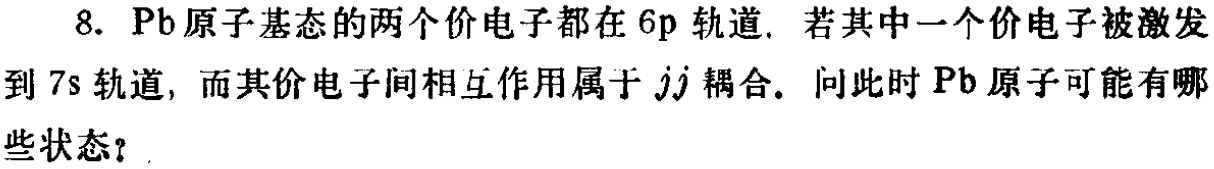
\includegraphics[width=\linewidth]{figures/Problem8}
  \label{fig:}
\end{figure}


jj coupling has 20 states as follows, as well

\begin{center}
\begin{tabular}{ Sc|Sc Sc } 
        & $j_1 = \dfrac{3}{2} $ & $j_1 = \dfrac{1}{2} $ \\
  \hline
  $j_2 = \frac{1}{2} $ & $J = 2,1$ & $J = 1,0$ \\ 
\end{tabular}
\end{center}

\end{document}